%-------------------------
% Rover Resume - Star Template
% Link: https://github.com/subidit/rover-resume
%
% CUSTOM COMMANDS \aux{} and \rside{} for part formatting
% eg. \subsection{Company Name \aux{Designation} \rside{Duration}}
% Double lined titles with \subsection{} and \subsubsection{}
% \linkicon gives external link icon
%-------------------------

\documentclass[11pt]{article}
\usepackage[T1]{fontenc}
\usepackage[utf8]{inputenc}

\usepackage[sfdefault,semibold,lf]{FiraSans}
\usepackage[a4paper,hmargin=1.8cm,top=1.3cm,bottom=1.7cm]{geometry}

\usepackage{xcolor}
\definecolor{accent}{HTML}{141E61}

\newcommand{\linkicon}{
  \color{gray}{\footnotesize\raisebox{1pt}{\faIcon{external-link-alt}}}
}

\setcounter{secnumdepth}{0}
\pdfgentounicode=1


%====== LIST FORMATTING ======
\usepackage{enumitem}
\setlist[itemize]{nosep, left=0pt .. 1.5em}
\setlist[enumerate]{left=0pt..1.5em}
\setlist[description]{itemsep=0pt}


%====== TITLE FORMATTING ======
\usepackage{xhfill}
\usepackage{soul}
\newcommand{\midrule}[1]{
  \leavevmode
  \xrfill[.5ex]{1pt}[accent]~\so{#1}~\xrfill[.5ex]{1pt}[accent]
}

\usepackage{titlesec}
\titlespacing{\section}{0pt}{*1.5}{*0.8}
\titlespacing{\subsection}{0pt}{*1.5}{*0}
\titlespacing{\subsubsection}{0pt}{*0}{*0}
\titleformat{\section}{\large\bfseries\uppercase}{}{}{\midrule}
\titleformat*{\subsection}{\large\bfseries\scshape}


%====== CUSTOM COMMANDS ======
\newcommand{\aux}[1]{
  $|$ \space {\normalfont\itshape #1}%
}

\newcommand{\rside}[1]{
  \hfill {\normalfont\color{accent} #1}%
}


%====== FOOTER ======
\usepackage{lastpage}
\usepackage{fancyhdr}
\pagestyle{fancy}
\fancyhf{}
\renewcommand{\headrulewidth}{0pt}

\fancyfoot[C]{\footnotesize\color{gray} I authorise the processing of my personal data in accordance with Regulation (EU) 2016/679 (GDPR) and Italian Legislative Decree 196/2003.}

% \pagestyle{empty} 
% uncomment previous line to hide page numbering


%====== PACKAGES ======
\usepackage{fontawesome5}
\usepackage{multicol}
\usepackage{graphicx}
\usepackage{tikz}
\usepackage[bookmarks=false,hidelinks]{hyperref}
\usepackage[protrusion=true,expansion=true]{microtype}


%====== FINISH PREAMBLE ======

%====== DOCUMENT STARTS HERE ======

\begin{document}

%====== BANNER ======

% Photo: overlaid on the left, the text stays centered on the page.
% For a version without photo, comment out the \makebox line with the photo block.
\noindent
\makebox[0pt][l]{%
\begin{minipage}[c]{3cm}
  \begin{tikzpicture}
    \clip (0,0) circle (1.35cm);
    \node at (0.2,-0.05) {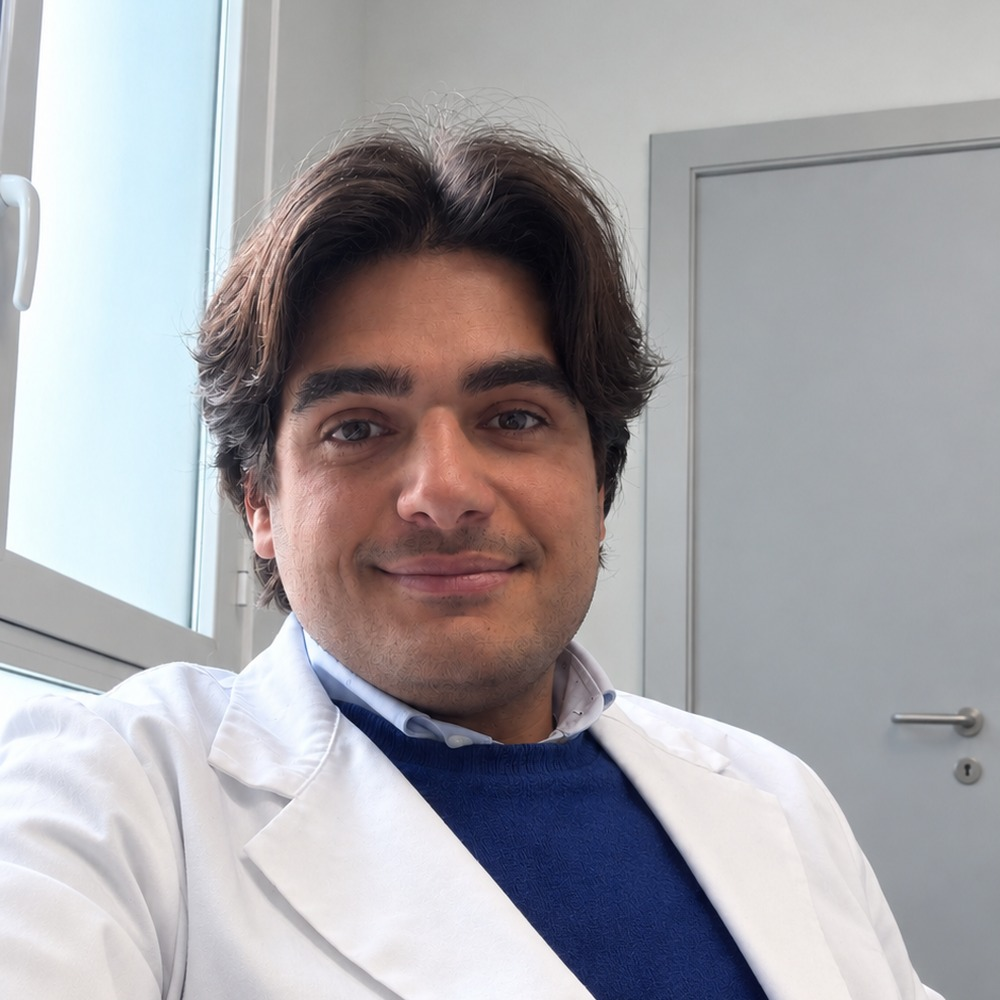
\includegraphics[width=3.4cm]{sagoma.jpeg}};
  \end{tikzpicture}
\end{minipage}}%
\begin{minipage}[c]{\linewidth}
  \centering
  {
    \fontsize{36}{12}
    \fontseries{heavy}\selectfont
    \color{accent}
    Simone Tringali % YOUR NAME HERE
  } \\ \medskip

  {\large MSc in Human Nutrition Sciences} \\ \medskip

  \href{tel:+393281639295}{{\color{gray}{\faPhone}} +39 328 163 9295} \quad
  \href{mailto:simone.tringali.96@gmail.com}{{\color{gray}{\faEnvelope}} simone.tringali.96@gmail.com} \\ \smallskip
  {\color{gray}{\faHome}} Palermo, Italy \quad
  {\color{gray}{\faCalendar*}} 02/02/1996 \quad
  {\color{gray}{\faCar}} Driving licence (B)
\end{minipage}

%====== BANNER END ======


\section{About me}
%==========
\noindent \textbf{Human Nutrition Sciences} graduate (MSc, LM-61, cum laude), with a bachelor's background in \textbf{Agri-Food Science and Technology}. Internship experience in \textbf{clinical nutrition} (bariatric surgery and oncology), assessing nutritional status and developing \textbf{personalised meal plans}. Skilled in \textbf{food quality and safety}, with a focus on \textbf{nutrition in intestinal disorders} developed in my thesis on irritable bowel syndrome. Preparing for the Italian \textbf{State Exam to qualify as a Biologist} (November 2026 session).

\section{Experience}
%==========
\subsection{Casa di Cura Macchiarella \rside{Palermo}}
\subsubsection{Nutrition Intern \rside{Feb 2026 -- Apr 2026}}
\begin{itemize}
  \item Assisted the clinic's nutritionist in \textbf{bariatric surgery} (pre- and post-operative) and \textbf{medical oncology} consultations.
  \item Dietary history, anthropometric measurements and body composition assessment with \textbf{bioelectrical impedance analysis (BIA)}; energy requirement calculation and \textbf{personalised nutrition plans}.
  \item Counselling for oncology patients and nutritional status assessment (\textbf{MNA}), within a \textbf{multidisciplinary team}.
\end{itemize}

\subsection{Istituto Sperimentale Zootecnico per la Sicilia \rside{Palermo}}
\subsubsection{Laboratory Analyst Intern \rside{Jan 2023 -- Feb 2023}}
\begin{itemize}
  \item Raw milk analysis with the \textbf{Combifoss 7} system (sample preparation, \textbf{data quality} checks) and monitoring of \textbf{quality parameters}: somatic cells, \textbf{ketosis}, \textbf{adulteration}.
\end{itemize}

\section{Education}
%==========
\subsection{Università Telematica San Raffaele \rside{Rome}}
\subsubsection{MSc in Human Nutrition Sciences (LM-61) \aux{110/110 cum laude} \rside{2024 -- 2026}}
\begin{itemize}
  \item \textbf{Thesis:} \textit{The role of diet in irritable bowel syndrome: current perspectives between clinical nutrition and food technology}.
  \item \textbf{Key subjects:} metabolic syndrome and intestinal diseases; eating disorders and hormonal regulation; food intolerances, immunity and drugs; nutritional analysis methods.
\end{itemize}

\subsection{University of Palermo \rside{Palermo}}
\subsubsection{BSc in Agri-Food Science and Technology \rside{2018 -- 2024}}
\begin{itemize}
  \item \textbf{Key subjects:} microbiology of food and fermented products; food technology; nutraceutical chemistry and nutrient metabolism; food hygiene and inspection.
\end{itemize}

\section{Continuing education}
%==========
\begin{itemize}
  \item \textbf{BIA START: understanding and interpreting the BIA method} \aux{Akern Academy} \rside{2026}
  \item \textbf{The malnourished patient: a challenge for the nutritionist} \aux{SIFA, online} \rside{2026}
  \item \textbf{Incretin therapy and precision nutrition in obesity} \aux{SIFA, online} \rside{2026}
  \item \textbf{Managing side effects of incretin-mimetic drugs} \aux{SIFA, online} \rside{2026}
\end{itemize}

\section{Languages and interests}
%===============
\begin{itemize}
  \item \textbf{Languages:} Italian (native); English B1 (intermediate).
  \item \textbf{Interests:} I am passionate about the link between \textbf{food}, \textbf{health} and \textbf{well-being}, which I carry beyond my studies: in the \textbf{kitchen} I experiment with recipes and \textbf{doughs}, putting into practice what I have learned about ingredients and food technology. I play team sports such as \textbf{football} and \textbf{padel} and keep up with \textbf{digital innovation}.
\end{itemize}



% \section{Certifications}
% %=======================
% \begin{enumerate}[label=\null, left=0pt..0pt, itemsep=0pt]
%   \item Some programming bootcamp, Location. \rside{2023}
%   \item Forbes Top 15 Procrastinators under 15. \rside{2022}
%   \item Perticipation award for attending workshop. \rside{2021}
% \end{enumerate}


% \section{Publications}
% %=====================
% \begin{enumerate}
%   \item A. Vaswani et al., “Attention is All you Need,” arXiv (Cornell University), vol. 30, pp. 5998 – 6008, Jun. 2017, [Online]. Available: \url{https://arxiv.org/pdf/1706.03762v5}
%   \item C. Darwin and J. Murray, \textit{On the origin of species by means of natural selection, or, The preservation of favoured races in the struggle for life.} 1859. doi: 10.5962/bhl.title.82303.
% \end{enumerate}


% \section{Awards}
% %===============
% \begin{description}
%   \item [2023] Some programming bootcamp, Location.
%   \item [2022] Forbes Top 15 Procrastinators under 15.
%   \item [2021] Conducted workshop on family planning by abstainance in SomePlace.
% \end{description}


% \section{Projects}
% %=================
% \subsection{Lunar Rover Project \aux{\href{https://robotics.nasa.gov/lmr/}{Link \linkicon}} \rside{2012 -- 13}}
% \begin{itemize}
%   \item LIDAR array, GPS, Variable FOV camera, Python, C/C++
%   \item Designed the rover to be modular, reconfigurable for sensor systems, handle science payloads, storage space, surplus resources, and robotics addons. % These modules shall be supported by centralized power and data ports. 
% \end{itemize}

% \subsection{Mars Rover \aux{\href{https://science.nasa.gov/mission/mars-exploration-rovers-spirit-and-opportunity/}{Project link \linkicon}} \rside{Feb 2012}}
% \begin{itemize}
%   \item Tech used, Language, Frameworks etc.
%   \item Implemented ABC feature
%   \item Optimised XYZ by 50\%
% \end{itemize}


\end{document}